\chapter{Recomendaciones generales}
\label{cap:Recomendaciones}

% [Autores: María José Rodríguez Fórtiz, Juanma, Alberto]
%%%%%%%%%%%%%%%%%%%%%%%%%%%%%%%%%%%%%%%%%%%%%%
%%%%%%%%%%%%%%%%%%%%%%%%%%%%%%%%%%%%%%%%%%%%%%

\section{Sobre la elección del TFG}

%%%%%%%%%%%%%%%%%%%%%%%%%%%%%%%%%%%%%%%%%%%%%%
%%%%%%%%%%%%%%%%%%%%%%%%%%%%%%%%%%%%%%%%%%%%%%

Ya estás en cuarto del grado y en ese momento aparece una asignatura de segundo semestre que se denomina Trabajo Fin de Grado de la cual sabes poco, salvo que tienes que realizar un proyecto. Te matriculas en ella y seguidamente se te vienen a la cabeza una serie de cuestiones, entre las que estarán seguro algunas de estas: ¿y ahora qué hago? ¿qué TFG elijo? ¿con qué docente? Normalmente vienen seguidas de un tiempo de cierta incertidumbre y algo de ansiedad, hasta que por fin consigues tener un tutor o tutora y un proyecto en el que ponerte a trabajar. En esta sección vamos a hacerte algunas recomendaciones para ayudarte a responderlas, y a que este proceso previo sea más llevadero.

Antes de comenzar, comentarte que existen dos fases en la asignación de TFG, (al menos en la ETSIIT). En la primera, el estudiante y el docente llegan a un acuerdo y en la segunda hace una preasignación del TFG al estudiante. En ella, el centro publica una lista de TFG que han propuesto los docentes y los estudiantes que no tienen TFG preasignados en la primera fase, eligen por orden de preferencia propuestas de TFG. El centro se encarga de realizar la asignación aplicando los criterios que estén vigentes en el momento (normalmente expediente académico de los estudiantes). Este proceso se suele realizar en octubre y en febrero o marzo. Todo esto, bajo la premisa de que estés matriculado en la asignatura. Que no se te olvide. También puede darse el caso de buscar TFG aunque no lo estés, porque quieras ir avanzando en el desarrollo del mismo. 

La primera sugerencia que te hacemos es que seas proactivo en la elección de la temática del TFG. No esperes a la segunda fase y busca tu TFG en la primera. No seas tímido y propón cambios a la idea que esté propuesta por el docente. El profesorado puede no querer cambiar su idea inicial, pero por lo general, a la hora de proponer TFG hay bastante flexibilidad. Se pueden proponer ideas nuevas, basta con hablar con algún docente que quieras que te tutorice. El hecho de que tú puedas proponer un TFG es un hecho fundamental en este proceso que impulsará  tu motivación, tu implicación personal y la originalidad del proyecto. Te permitirá explorar áreas de interés genuino que a menudo se traducen en investigaciones o desarrollos más profundos, creativos y alineados con las vocaciones y aspiraciones profesionales que puedas tener.

Respecto a cuándo empezar, aunque es una asignatura de segundo semestre muchos estudiantes comienzan a buscar y trabajar en él en el primer semestre o a final de tercero. Así, hay ocasiones en que los estudiantes tenéis muy claro qué queréis hacer en vuestro TFG. Esto puede deberse a múltiples situaciones. Por ejemplo, imagina algunas de estas: desde algunos cursos antes tienes entre manos el desarrollo de un proyecto personal y consideras que el TFG puede ser un contexto idóneo para avanzarlo; o bien, lo que tienes es una idea de proyecto personal y esta asignatura te plantea una excusa perfecta para llevarlo a cabo. También puede ser que hayas aprendido alguna tecnología o aplicación en alguna asignatura y estás motivado para trabajar en ella. Pero no sólo tienen que ser proyectos personales, sino que también entra en juego tu mentalidad emprendedora: has detectado un nicho donde el producto o servicio que obtengas como salida de tu TFG es susceptible de ser comercializado. Y también están los proyectos profesionales. Es habitual que cuando llegues a cuarto estés haciendo tus prácticas en empresa o incluso que ya estés contratado. Y en ese entorno profesional pueden existir desafíos o temáticas en las que estás trabajando en tu empresa, o podrías trabajar, y que serían susceptibles de ser abordados en tu TFG.

Asumiendo que estás en una de estas situaciones, o en cualquier otra en la que ya tengas una idea clara de lo que quieres hacer, el primer paso que tienes que dar es sentarte tranquilamente y escribir una descripción del problema que deseas abordar, lo suficientemente completa para que un posible lector tenga una idea bastante clara de tu propuesta. 

El siguiente paso será la búsqueda del docente que te dirigirá el trabajo. Aquí existen varias situaciones: la primera es que tienes cierta confianza con algún docente o cierta afinidad personal, te cae bien o crees que puedes trabajar bien con él o ella. En ese caso, concierta una tutoría y exponle tu idea, y dile directamente que te gustaría que fuera la persona que te tutorice, explicándole las razones. Ese documento que habías hecho, házselo llegar previamente a la tutoría con objeto de que conozca tu idea y puedas explicársela con cierto conocimiento de la misma por su parte y resolver las dudas que te pueda plantear. Si te dice que sí, has triunfado y, a partir de ahí, os podéis poner a trabajar, seguramente en una fase inicial en la que concretéis detalles del proyecto. Si te dice que no, busca otro docente. Podría ser interesante que hicieras una lista con los docentes a los que plantearle la tutorización, ordenada por preferencia. La otra alternativa para solicitar a un docente que sea la persona que te tutorice es que sea experto en la temática de tu idea. En este caso, busca qué profesorado investigan en ese tema o imparten clases en asignaturas relacionadas, y procede de la misma forma explicada. Para ello, inspecciona las guías docentes de las asignaturas afines a la temática de tu idea, mira los sitios web de los departamentos y de los grupos de investigación para encontrar docentes que sean expertos en temas relacionados con tu idea. 

Si no tienes una idea clara, pero sí sabes con certeza con qué tutor querrías trabajar, concierta una cita y dile que quieres hacer el TFG con él o ella, y si existe la posibilidad de que te proponga algún tema que pueda ser de tu interés. Si dice que sí, y hay alguna propuesta que te guste, ya puedes empezar a trabajar. Si dice que no o ninguna de las propuestas te interesan, entonces echa mano del siguiente docente de la lista.

Otra opción que existe cuando no se tiene una idea clara de lo que hacer y tampoco se tiene claro con quién hacerlo es acudir a la web donde se publican las propuestas de TFG para ese curso. Como te hemos comentado, en la primera fase los docentes suelen publicar sus propuestas con objeto de darlas a conocer y que los estudiantes las puedan elegir. Mira las que te gustan y cítate con los docentes para que te las expliquen con más detalle. Cuando encuentres una propuesta que te guste, solicítasela al profesor. 

Todo lo anteriormente indicado se aplica en la fase de preasignación. Si por cualquier causa (despiste, falta de iniciativa, dudas, etc.) no se te ha asignado un TFG en esta fase, pasarías a la segunda. Como ya hemos comentado, tendrás que ordenar los TFG propuestos que han quedado sin asignar en orden decreciente de interés, y esperar que el centro te asigne alguno de los que has seleccionado. En este caso, no hagas la ordenación al tuntún ni introduzcas en la lista todos los TFG. En su lugar selecciona los que verdaderamente te interesen. Habla con los tutores o tutoras de los que te gustan y pídeles que te den detalles para que puedas hacer una ordenación informada según tus gustos, combinando tanto la temática del TFG como el docente que lo propone. A partir de ahí, a cruzar los dedos para que el que has puesto como primero, o alguno de los primeros puestos, sea el que se te asigne. Corres el peligro de que te den uno situado al final de esa lista. Esto tiene al menos dos inconvenientes: puede ser que no te motive la propuesta o que la persona que te tutoriza que te ha tocado no sea santo de tu devoción. En ese caso, tendrás que plantearte si seguir para delante con lo que te ha tocado o dejar el TFG para el curso siguiente (no tiene que ser junio, también puede ser la convocatoria extraordinaria, normalmente en noviembre) y buscar o proponer tú el tema de tu TFG con tiempo.

Como podrás imaginar, siempre es mejor que tengas tú la iniciativa y buscar una proyecto que te motive y un tutor o tutora con quien estés a gusto trabajando. Piensa que las horas las tienes que trabajar igualmente, así que mucho mejor si lo haces persiguiendo un objetivo que te interese y motive.

También es importante, si optas por la la opción proactiva, el momento en el que comienzas a moverte y a realizar contactos con el profesorado. Si lo dejas para muy tarde, seguramente éstos estén ya cargados de TFG y puedas recibir varias negativas a tus propuestas o los propuestos que te interesan ya hayan sido preasignados. Si es así, no te vengas abajo. Ten en cuenta que no es algo personal. Esta es la razón por la que te recomendamos que comiences el proceso de búsqueda de TFG lo antes posible. Hay estudiantes que a final de tercero, antes de vacaciones, están buscando ya; otros justo a la vuelta, en septiembre, y algunos lo dejan para la asignación de noviembre o febrero. En este último caso, las opciones quedarán reducidas considerablemente, así que, cuanto antes mejor.

En esas reuniones previas a la preasignación en las que finalmente hay un acuerdo entre estudiante y docente, un aspecto muy relevante es la discusión del alcance del TFG y sus objetivos. En ellas tenéis que concretar cuáles serán las funcionalidades de los desarrollos asociados al TFG y qué objetivos os marcáis para el mismo. Estas negociaciones son importantes porque determinarán hasta dónde tendrás que llegar en tu proyecto. En este sentido, cuando se te preasigne asegúrate de que tengas claro este alcance. Procura, al definir estos objetivos, que sean realistas, y que consideres para que así sean, el tiempo que tienes disponible para trabajar en él y cuándo quieres tenerlo listo para entregarlo. De todas formas, los objetivos pueden ir cambiando a lo largo del desarrollo.

Puedes ver un resumen de todo este proceso en la figura  \ref{fg_diagrama_proceso}.

Para concluir esta sección, comentarte que la realización de un TFG es un proceso que te está entrenando para el ámbito profesional. Vas a realizar un trabajo que se asemejará al que realizarás cuando hayas terminado y estés contratado en una empresa. Aprovecha esta oportunidad para aprender nuevas metodologías, tecnologías, lenguajes, etc. que no has visto en el grado y que te puedan servir en la nueva fase profesional que se te abrirá en pocos meses. Además, es una magnífica carta de presentación en las entrevistas ya que podrán ver tu capacidad de trabajo y de aprendizaje de nuevos conceptos, cosa que permitirá diferenciarte de otros candidatos. Por tanto, te sugerimos que aproveches la oportunidad de realizar un TFG en el que aprendas muchas cosas y en una temática que te guste. 

Como nota final, recuerda que para presentarlo en la convocatoria extraordinaria de noviembre tienes que haberlo solicitado en la \url{sede.ugr.es} tal y como indica {la web de la ETSIIT}\footnote{\url{https://grados.ugr.es/informatica/pages/infoacademica/tfggestion2}}. Hay unos plazos para dicha solicitud, no dejes que se te pase.

% SUGERENCIA -> INFOGRAFÏA CON DIAGRAMA DE FLUJO DEL PROCESO
\begin{figure}[!ht]
\centering
    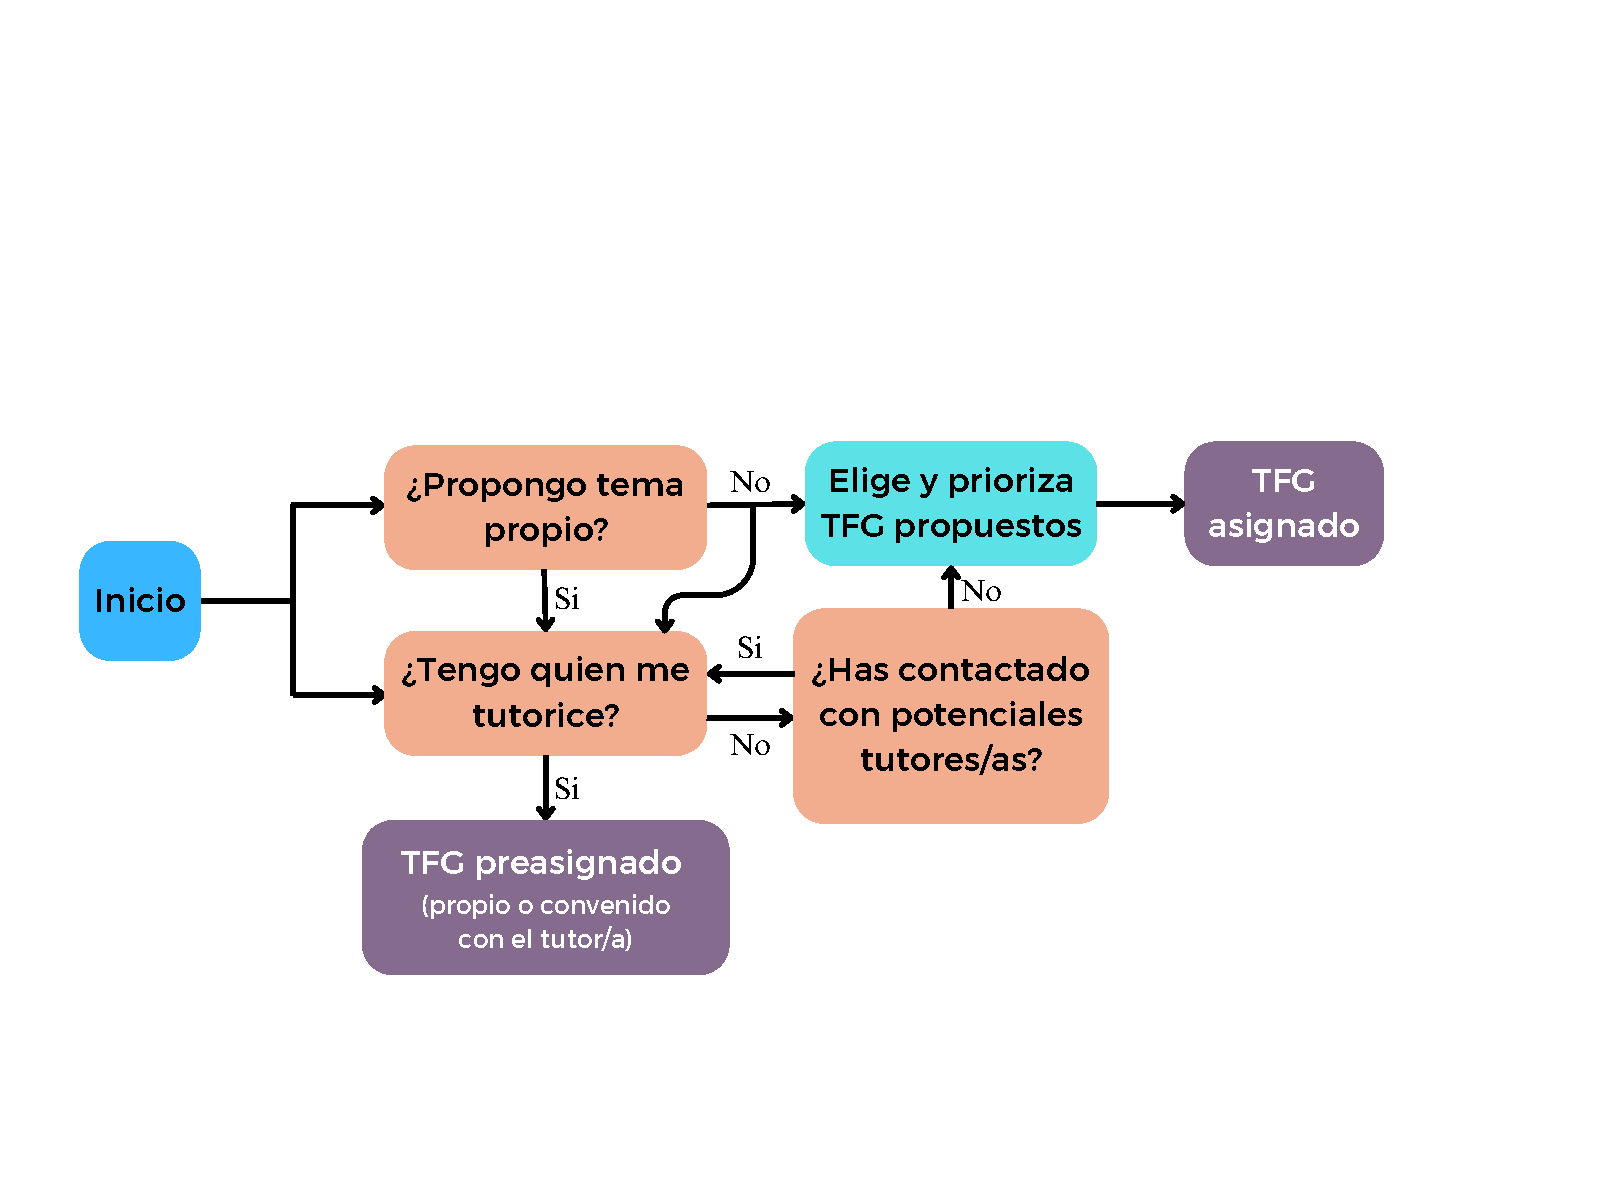
\includegraphics[scale=0.5]{images/DecisionTFG.pdf}
    %\alt{Diagrama que parte de una solicitud de TFG hasta su asignación o presasignación}
    \caption{Diagrama de flujo del proceso.}\label{fg_diagrama_proceso}
\end{figure}

%%%%%%%%%%%%%%%%%%%%%%%%%%%%%%%%%%%%%%%%%%%%%%
%%%%%%%%%%%%%%%%%%%%%%%%%%%%%%%%%%%%%%%%%%%%%%

\section{Sobre el desarrollo del proyecto}

%%%%%%%%%%%%%%%%%%%%%%%%%%%%%%%%%%%%%%%%%%%%%%
%%%%%%%%%%%%%%%%%%%%%%%%%%%%%%%%%%%%%%%%%%%%%%

En esta sección vamos a comentar aspectos fundamentales para el éxito de cualquier proyecto. Comenzaremos con la comunicación con la persona que te tutoriza, posteriormente con la disciplina y la pauta de trabajo (no es lo mismo caminar un kilómetro cada día durante cien días que caminar cien kilómetros en un día...), y cuestiones menos técnicas como aspectos éticos y de propiedad intelectual.

%%%%%%%%%%%%%%%%%%%%%%%%%%%%%%%%%%%%%%%%%%%%%%
\subsection{Reuniones con la persona que te tutoriza}%(María José)
%%%%%%%%%%%%%%%%%%%%%%%%%%%%%%%%%%%%%%%%%%%%%%

Durante el desarrollo del TFG debes mantener varias reuniones con la persona que te tutoriza con el objetivo de organizar y revisar tu trabajo. Las reuniones pueden ser presenciales u \textit{online}, dependerá de ambos.

En las primeras reuniones con la persona que te tutoriza, tal y como se ha comentado antes, debes consensuar el alcance y objetivos del proyecto. Un TFG debe ser un trabajo original, claro, riguroso, coherente, relevante, y pertinente. Por eso, te insistimos en que concretes bien y sin divagar cuál va a ser la orientación y aportación del trabajo desde el principio, qué se va a mejorar respecto a lo existente. En las reuniones iniciales también se debe proponer y seleccionar la metodología a seguir y cuál será la estructura de la memoria. Aunque luego pueda haber cambios, es interesante hacer el ejercicio a priori para tener una idea de cómo se va a desarrollar el trabajo.

En las siguientes reuniones la persona que te tutoriza puede ayudarte a resolver dudas, ir validando el desarrollo realizado, y corregir lo que vayas escribiendo de la memoria, por ejemplo, indicándote el grado de profundidad al exponer los temas, o las mejores herramientas de diseño a utilizar. También puede sugerirte bibliografía para completar el estado del arte o contexto del trabajo o incluso facilitarte materiales para el desarrollo. 

Te aconsejamos que te reúnas con la persona que te tutoriza con frecuencia, aunque esta varíe según tus otras ocupaciones en otras asignaturas o en tu trabajo, si ya lo tienes. Lo habitual es quedar de forma sistemática con ella en diferentes momentos considerando la metodología de trabajo que estés siguiendo, al acabar un paso, fase o tarea, y antes de empezar el siguiente. Eso te obligará a ser más constante en tu trabajo ya que sabes que tienes que rendir cuentas de lo que has hecho en ese tiempo. Así, por ejemplo, es frecuente planificar pasos, fases o tareas de dos semanas, y tener las reuniones también con esa frecuencia. Si prevés que vas a estar un tiempo sin poder trabajar en el TFG, hazlo saber a la persona que te tutoriza para planificar reuniones a más largo plazo. Del mismo modo, si requieres reuniones más frecuentes, házselo saber para llegar a un acuerdo. 

Te aconsejamos también que planifiques bien cada reunión, y determines qué quieres mostrarle y qué consultar. Si es posible, envíale material resultante de tu trabajo antes de la reunión para que tenga tiempo de mirarlo. En ese caso, la reunión será más efectiva, centrándose en los comentarios que tenga sobre tu entrega y en tus dudas. Otros consejos son que te vayas apuntando esas dudas que te surjan conforme vayas trabajando para llevarlas a la siguiente reunión, y que tomes acta (apuntes) de lo que se hable en la reunión, o incluso la grabes si la persona que te tutoriza está de acuerdo. De ese modo podrás repasarlo todo después. 

De hecho, igual que recomendamos tener una bitácora para el desarrollo, también puedes incluir en ella estas reuniones (o crear una por separado). De ese modo, queda constancia del trabajo continuo a lo largo del tiempo y tanto tú, como el tutor, como el tribunal calificador pueden ver la evolución del trabajo y validar la planificación.

Las reuniones estrechan los lazos tutor-estudiante, ten confianza para exponer tus dudas, falta de tiempo o motivación, para que se puedan resolver los problemas cuanto antes. Si tienes desacuerdos con la persona que te tutoriza, justifica tu postura, eres tú el que estás realizando el trabajo y el que llegado un momento puede conocerlo mejor, así que haz un esfuerzo por argumentar tus decisiones. 

En el extraño caso de que haya una diferencia de opinión irresoluble con tu tutor, siempre desde la corrección y el respecto, puedes recurrir al coordinador de la titulación para que te asesore y ver cómo proceder. 

%%En el caso de que no llegues a tener esa confianza con la persona que te tutoriza o no estés recibiendo la supervisión que necesitas, te aconsejamos que lo hables y si no se le da solución, que busques apoyo en tus compañeros u otros profesores/as.

Por último, hacerte saber que las reuniones son la herramienta que la persona que te tutoriza tiene para evaluar tu trabajo y éste hará una evaluación continua de él. Recuerda que quien te dirige tu trabajo pone parte de la nota final, así que debes mantenerla informada de lo que vas haciendo, hacerle entregas y realizar mejoras sobre entregas previas teniendo en cuenta sus sugerencias. Si la persona que te tutoriza percibe que vas a las reuniones sin realizar el trabajo planificado, que si vas no estás atento o no tomas nota, que en las entregas no tienes en cuenta sus sugerencias o no argumentas porqué, no puedes esperar una gran calificación, aunque luego entregues una memoria final ``estupenda''.

%%%%%%%%%%%%%%%%%%%%%%%%%%%%%%%%%%%%%%%%%%%%%%
\subsection{Disciplina/pauta de trabajo}% (María José)
%%%%%%%%%%%%%%%%%%%%%%%%%%%%%%%%%%%%%%%%%%%%%%

El TFG se realiza durante varios meses, lo que requiere de una planificación del trabajo a corto y largo plazo. 

Si eres una persona disciplinada, no te costará trabajo hacer un calendario semanal en el que busques unos huecos para el TFG y para reuniones con la persona que te tutoriza, de tal forma que puedas hacer tu trabajo de manera progresiva. 

Sin embargo, si eres una persona con tendencia a la procrastinación (dejarlo todo para el último día para trabajar con presión), es el momento de que busques apoyos para evitar esto, ya que te aseguramos que así no podrás hacer el TFG. Te aconsejamos que te organices, que establezcas prioridades y que dividas tu trabajo en tareas más pequeñas que puedas realizar con menos esfuerzo. Ponte un horario planificando descansos y trabaja siempre en el mismo sitio, con una mesa de trabajo limpia y sin distractores. Utiliza aplicaciones de agenda y gestión del tiempo que te avisen de cuándo hay que hacer cada tarea, y programa un tiempo de finalización para que no te distraigas. Por ejemplo, aplicaciones como {Trello}\footnote{\url{https://trello.com/}} o {FocusToDo}\footnote{\url{https://www.focustodo.cn/}} ayudan a ello. Otra alternativa para combinar tanto la bitácora como un panel de tareas que se transforma en un Diagrama de Gantt en {Notion}\footnote{\url{https://www.notion.so/}}. Si necesitas más apoyo aún, busca herramientas con ``gamificación'' que te impidan distraerte y te den premios al finalizar tu trabajo, como {Forest}\footnote{\url{https://www.forestapp.cc/}}, o dátelos tú mismo/a para tener un refuerzo positivo que te ayude a seguir adelante y mantener esa dinámica. 

%Alberto 
Para cuantificar el tiempo que le dedicas, medir tu avance y llegar a las 300 horas que, como mínimo, se deben invertir en el TFG puedes cronometrar el tiempo dedicado mediante aplicaciones como {Clockify}\footnote{\url{https://clockify.me/es/}} y también puedes guardar un log o bitácora donde puedes incluir un párrafo resumiendo lo avanzado en ese intervalo de tiempo que has dedicado. El ejercicio de resumir lo que has avanzado te ayudará a avanzar e incluso a resolver algún problema que te haya surgido. No te desanimes si, en ocasiones, no tienes mucho que escribir, el poder transmitir conocimiento no es sencillo y puede requerir que discurra un tiempo hasta que puedas hacerlo. Lo que está claro es que si no te sientas a escribir esa bitácora, muy probablemente nunca llegues a desarrollar esa capacidad, en palabras atribuidas, entre otros a Picasso: {\it ``Si llegan las musas, que te pillen trabajando''} \footnote{\url{https://www.elcorreoweb.es/economia/2020/07/02/musa-pilla-trabajando-104593995.html}}

En el cómputo de las horas dedicadas, incluye también el tiempo invertido con el tutor desde la primera reunión hasta el posible ensayo de la presentación, el tiempo de buscar bibliografía, el tiempo que has dedicado a leer cosas relacionadas con el proyecto así como cualquier aspecto del desarrollo.

Si usas VSCode para escribir el código o la memoria del TFG, hay {\it plugins} que permiten controlar el tiempo dedicado. Por ejemplo {Waka}\footnote{\url{https://wakatime.com/vs-code}} proporciona uno. De este modo, se puede hacer una revisión de la cantidad de trabajo dedicada a cada funcionalidad y objetivo y evaluar la planificación realizada a priori.

%%%%%%%%%%%%%%%%%%%%%%%%%%%%%%%%%%%%%%%%%%%%%%
\subsection{Planificación y herramientas} %(María José)
%%%%%%%%%%%%%%%%%%%%%%%%%%%%%%%%%%%%%%%%%%%%%%
Una vez consensuados con la persona que te tutoriza cuáles van a ser los objetivos del TFG, lo primero que se debe hacer es planificar las tareas a realizar durante todo el proyecto, teniendo en cuenta una metodología de trabajo en la que habrá varios pasos o fases. Esa planificación deberá quedar reflejada en la memoria con objeto de mostrar cómo has organizado todo tu trabajo.

En tu TFG seguramente tendrás que realizar tareas de varios tipos, que podrán variar dependiendo el tipo de proyecto que estés realizando. Estos tipos principales de tareas son: revisión bibliográfica, aprendizaje de herramientas y tecnologías, desarrollo, reuniones, redacción de la memoria, y evaluación. Además, el propio desarrollo requiere también de una metodología de trabajo que variará según éste, pero que incluirá sus propias tareas. Todos estos tipos de tareas podrán aparecer en la planificación. Y en definitiva cualquier cosa que necesites hacer para conseguir los objetivos de tu TFG.

Te aconsejamos que, conociendo tu disponibilidad de tiempo, seas tú quien hagas la primera propuesta de planificación temporal que muestres al tutor, incluyendo tareas de todos los tipos mencionados arriba. La distribución de tareas la realizarás, como hemos indicado, teniendo en cuenta las metodologías a seguir, pero dependerá de ti y de la persona que te tutoriza el que alternes tareas más de desarrollo con otro tipo de tareas de aprendizaje, lectura de bibliografía y redacción. Esta alternancia puede ayudar a hacer el trabajo menos tedioso y evitar frustraciones si nos atrancamos en algún punto y nos permitimos pasar a otro tema mientras tanto. También puede ayudarnos a tener una conciencia de que estamos progresando un poco en todo. 

Respecto a la distribución de tareas, no aconsejamos que se haga el desarrollo al principio y se escriba la memoria después, sino que se haga al mismo tiempo, que conforme se van concretando las especificaciones y diseños, éstos vayan formando parte de la memoria. Tampoco aconsejamos empezar el desarrollo sin haber hecho una buena revisión de tecnologías y posibles herramientas a utilizar, y sin revisar aplicaciones o trabajos similares. Estas revisiones ayudarán a elegir las mejores herramientas y tecnologías, así como nos darán mejores ideas sobre cuál puede ser nuestra aportación sobre el estado del arte existente. Recuerda justificar siempre cada decisión tomada y, en caso de ser equivalentes, siempre tienes el comodín de indicar que no la conocías y preferías aprender sobre ella.

Para hacer una planificación debes cuantificar el tiempo que vas a dedicar a cada tarea. Cuanto más pequeña sea la tarea más fácil será calcular cuánto tiempo le debes dedicar, por lo que te sugerimos que llegues a la granularidad más fina que puedas. Organiza las tareas en un calendario semanal en el que también tengas programadas el resto de tus actividades, incluidas las personales. Procura que las tareas del TFG no interfieran en el resto de tus actividades y viceversa, manteniendo un equilibrio. No te pongas tareas del TFG en tiempo de exámenes, de entregas de otros trabajos, o de vacaciones. Planifica con holgura, considerando que puedas siempre tardar un poco más de lo que estimas, porque muchas veces surgen complicaciones e imprevistos (sobretodo si tienes que aprender nuevas tecnologías) y es mejor contar con ese tiempo por si acaso 

A lo largo del desarrollo del proyecto, procura seguir el cronograma que has fijado. Revisa tu ajuste a las fechas con frecuencia y en el caso de que haya desviaciones frente a la estimación inicial, haz cambios en la planificación inmediatamente. Los motivos más frecuentes de desvío pueden ser que no se haya hecho una buena estimación inicial, que haya cambios en el alcance (requisitos u objetivos) del proyecto, que haya problemas con las tecnologías o herramientas elegidas para el desarrollo, que no se sea tan productivo como se pensaba, etc. Es muy raro que en algún proyecto no haya que hacer ajustes y por ello hay que considerarlos realizando actuaciones que mitiguen el retraso. Los ajustes pueden ser temporales o de alcance del proyecto. Ejemplos de ajustes temporales que podrías hacer son: intensificar el ritmo de trabajo en las próximas semanas, reorganizar el cronograma para optimizar la utilización del tiempo restante, o priorizar tareas críticas para asegurar la entrega de lo más relevante en plazo. En cuanto a ajustes relacionados con el alcance del proyecto estarían los siguientes:  replanificar objetivos, eliminar tareas o subtareas menos prioritarias, redefinir el enfoque de alguna parte del trabajo, o incluso reordenar las prioridades globales del proyecto para enfocarse en los aspectos más esenciales y viables dentro del tiempo disponible. Consensúa con la persona que te tutoriza qué hacer en función del motivo del desajuste y el estado del TFG. Esto es importante, ya que si no tomas consciencia a tiempo de que vas con retraso en tu trabajo y no tomas medidas, ese retraso puede hacer que no termines el TFG a tiempo de su entrega, pese a haber dedicado mucho tiempo a él. 

Es un gran ejercicio reflexionar sobre las causas de los desajustes y aprender de ellos para futuros proyectos. Piensa que los cambios y ajustes que hagas constituyen en realidad una oportunidad de aprendizaje y un reflejo de la dinámica de la investigación y el desarrollo que se hace en la realidad. Por eso mismo, es importante que justifiques los cambios de forma positiva en la memoria del TFG. De hecho, la capacidad de identificar contingencias, adaptarse a los cambios y gestionar imprevistos es una competencia muy valiosa en cualquier ámbito profesional y académico. Puedes ir indicando en la memoria cuál ha sido la replanificación realizada en cada fase del proyecto, añadiendo las causas de los cambios y cómo se han repensado las tareas. También puedes mostrar tu planificación inicial y el cronograma final, explicando con un párrafo los principales cambios y ajustes realizados.

Para realizar tu planificación temporal puedes usar herramientas como los diagramas de Gantt. Hay muchas aplicaciones gratuitas que te facilitan su realización, y muchas de ellas te ayudan a hacer ajustes y cambios, o incluso simulaciones sobre una línea base, para ayudarte a tomar decisiones sobre las mejores opciones. Otra posibilidad que integran muchos gestores de proyectos es definir las tareas con la estimación de tiempo y, automáticamente, ellos generan el diagrama.

% Alberto -> me lo he llevado a Pauta de trabajo. Aparte de esto, te aconsejamos que tomes nota de forma sistemática del tiempo que dedicas al trabajo y en qué tareas. Esto te ayudará a hacer un cálculo final del presupuesto del proyecto, cuantificando el coste de tu trabajo por hora. También te permitirá ver cómo es tu productividad y comparar tu dedicación a diferentes tipos de tareas. Existen herramientas online como \href{https://clockify.me/}{Clockify} que ayudan a apuntar el tiempo dedicado a las tareas y generan varios tipos de informes, aunque también puedes usar una simple hoja de cálculo si lo prefieres.

%%%%%%%%%%%%%%%%%%%%%%%%%%%%%%%%%%%%%%%%%%%%%%
\subsection{Cuestiones éticas y legales}% María José
%%%%%%%%%%%%%%%%%%%%%%%%%%%%%%%%%%%%%%%%%%%%%%

A la hora de preparar el TFG y de redactar la memoria hay que tener en cuenta varios aspectos éticos y legales.

Si en tu TFG vas a hacer algún experimento docente o de salud que implique seres humanos, los principales principios éticos a considerar son los de garantizar el respeto de opiniones, causar beneficio y no daño o perjuicio, y procurar justicia. El TFG es corresponsabilidad del estudiante y la persona que tutoriza, luego ambos debéis garantizar que se cumplan esos principios \cite{EticaCantabria}. 

Si en el TFG se va a hacer un estudio con datos sensibles de personas, como datos clínicos, se van a recoger muestras biológicas, o se va a trabajar con datos que les puedan identificar, es necesario que el estudio esté aprobado por el {Comité de Ética de la universidad}\footnote{\url{https://investigacion.ugr.es/informacion/presentacion/apoyo/comite-etica/evaluacion}}, solicitando una evaluación y preparando un consentimiento informado. El consentimiento informado es un documento que firma el participante (o un tutor legal si el participante es menor de edad) en el que se describe la naturaleza del estudio, se precisa el tipo de participación de las personas que formarán parte del estudio, y que el uso de los resultados será solo para fines docentes, y/o de investigación en su caso. Además, es obligatorio indicar que la participación es voluntaria y que se puede revocar en cualquier momento, sin tener que dar explicación. También se debe asegurar el anonimato de los participantes y la custodia de datos, todo ello recogido por la {Ley Orgánica de Protección de Datos Personales y Garantía de Derechos Digitales- LPDGDD}\footnote{\url{https://www.boe.es/buscar/act.php?id=BOE-A-2018-16673}}. Según ésta, los datos sensibles de una persona, aparte de los datos médicos, son aquellos que permiten identificar su ideología, afiliación sindical, religión, orientación sexual, creencias u origen racial o étnico. También son sensibles los datos de contacto de las personas, dni, teléfono, dirección, etc., siempre y cuando no sean los de su localización profesional, si es necesaria. Si tu TFG recoge algunos de estos datos sensibles, debes seguir las indicaciones de la LPDGDD. Por ejemplo, si vas a acceder a historias clínicas, aseguraos de que los datos estén ya anonimizados y que son facilitados por personal sanitario acreditado, que actuará como supervisor. Si en tu TFG vas a usar grabaciones de vídeo o audio de personas, ten en cuenta que también son datos de carácter personal, luego también hay que pedir un consentimiento informado en estos casos. Si la recogida de datos se hace en un centro no universitario, debes contar además con autorización de ese otro centro para realizar el estudio.

En el caso de que hayas recogido datos sensibles como los mencionados, y tengas previsto difundir información de él, debes hacer esa difusión exclusivamente a través de los servicios de comunicación de la universidad, así como contar también con la autorización del centro donde se realice el estudio, si es externo a la universidad.

La UGR también considera que en un TFG hay otros aspectos éticos específicos a considerar, que son los siguientes \cite{EticaUGR}:
\begin{itemize}
    \item Valorar el impacto social y medioambiental de las soluciones técnicas que se proponen, comprendiendo la responsabilidad ética y social.
    \item Usar mecanismos que fomenten la igualdad y participación, rompiendo la brecha digital.
    \item Fomentar el espíritu crítico y transdisciplinar.
\end{itemize}

Si en tu TFG has tenido en cuenta algunos de esos aspectos, debes mencionarlos en la memoria, bien cuando planteas tu solución de diseño o arquitectura, o bien en las conclusiones.

Centrándonos en la ética informática, y según \cite{bynum2000}, ésta identifica y analiza el impacto de la tecnología en los valores sociales y humanos, por ser personas las que manipulan la tecnología. Las asociaciones de profesionales de informática y algunas empresas han elaborado códigos de conducta profesional (muchos de los cuales también están recogidos por la LPDGDD) para regular las nuevas tecnologías y orientar sobre principios específicos relacionados con la ética de su profesión, y que tú, como ya casi profesional de la informática, debes considerar tales como garantizar:  
\begin{itemize}
    \item Privacidad y disposición de información, gestionando el consentimiento en el uso de los datos por parte del participante, con derechos de acceso, rectificación, supresión, limitación del tratamiento, portabilidad y posición.
    \item Transparencia, seguridad y protección en la recolección, uso, procesamiento, transmisión y comunicación de información: exactitud, anonimización y minimización. 
    \item Uso de las alternativas tecnológicas menos invasivas para no interferir en los derechos de las personas.
    \item Responsabilidad sobre el trabajo realizado si se incumple alguna legislación, principalmente para no causar perjuicio económico, moral o social.
    \item Protección y respeto a los derechos de autor y propiedad intelectual, no plagiando sino citando el trabajo de otros.
\end{itemize}


Además de la LPDGDD, hay otras leyes que debes considerar al realizar tu TFG, por ejemplo:
 
\begin{itemize}
    \item Interoperabilidad: Real Decreto 203/2021, de 30 de marzo, por el que se aprueba el Reglamento de actuación y funcionamiento del sector público por medios electrónicos.
    \item El código Penal español (Ley Orgánica 5/2010, de 22 de junio, por la que se modifica la Ley Orgánica 10/1995, de 23 de noviembre), recoge los delitos informáticos, como el acceso no autorizado a sistemas informáticos, la interceptación de comunicaciones, la falsificación de documentos, la estafa informática, la difusión de virus informáticos, el sabotaje en sus artículos 197, 248, 264.
    \item Accesibilidad: Real Decreto 1112/2018, de 7 de septiembre, sobre accesibilidad de los sitios web y aplicaciones para dispositivos móviles del sector público.
\end{itemize}

Para evitar tener que consultar legislación y acuerdos internacionales, procura evitar cualquier servicio de terceros que no esté dentro de la Unión Europea. Por ejemplo, en el caso de un proveedor de nube, procura elegir una región que esté dentro de Europa.

En resumen, habría que seguir los mandamientos de ética que ya sugería \cite{EticaUCM} en 1992 y que siguen vigentes: no usar el ordenador para dañar a otras personas, robar, dar falso testimonio, plagiar o apoderase del trabajo de otros; pensar en las consecuencias del programa o sistema que se desarrolla (sobre todo si el sistema toma decisiones, realiza predicciones/clasificaciones, o genera datos, de forma automática); y garantizar siempre la consideración y el respeto hacia los semejantes.

Asegúrate de que tu TFG respete esos mandamientos y tenga en cuenta la legislación vigente.

Finalmente es importante conocer la normativa de tu universidad a la hora compartir la autoría de tu trabajo. En algunos casos, la autoría podría depender del grado de colaboración con la persona que te dirige, por lo que puede ser relevante establecer esta colaboración mediante la aplicación de licencias. Esto es especialmente importante en el caso de TFG realizados en colaboración con empresas. Para más información sobre Propiedad Intelectual y licencias, por favor, no dejes de consultar el anexo \ref{anexo:licencias}, donde presentamos la normativa de la UGR y te explicamos los distintos tipos de licencias, especialmente las libres y abiertas, que puedes aplicar a tu proyecto.

De cualquier forma, todos estos detalles deberían quedar claro con quien ejerce la tutoría de tu trabajo en las primeras reuniones del proyecto, aunque esto puede modificarse más adelante. 

%%%%%%%%%%%%%%%%%%%%%%%%%%%%%%%%%%%%%%%%%%%%%%
%\section{Sobre la propiedad Intelectual} %Esta sección completa puede ser un anexo
%%%%%%%%%%%%%%%%%%%%%%%%%%%%%%%%%%%%%%%%%%%%%%





%%%%%%%%%%%%%%%%%%%%%%%%%%%%%%%%%%%%%%%%%%%%%%
%%%%%%%%%%%%%%%%%%%%%%%%%%%%%%%%%%%%%%%%%%%%%%

\section{Sobre la redacción de la memoria} %Alberto

%%%%%%%%%%%%%%%%%%%%%%%%%%%%%%%%%%%%%%%%%%%%%%
%%%%%%%%%%%%%%%%%%%%%%%%%%%%%%%%%%%%%%%%%%%%%%

% añadido por María José en forma más o menos telegráfica, por completar por Alberto:
% - Resumen, debe ocupar una media página. Debe incluir varios párrafos que resuman:  el contexto o motivación, sus objetivos generales, la metodología seguida, las tecnologías o herramientas aplicadas, los resultados obtenidos y una conclusión sobre su aportación. Cuidado, que muchos resúmenes se quedan solo en el contexto y objetivos. Debe ser completo. El resumen debe hacerse al final. 
% - Índice, mejor hacerlo automático al final. Usando estilos para las secciones y párrafos. Numerado. 
% - Agradecimientos: a instituciones y personas
% - Introducción: motivación académica y científica de la pertinencia del TFG: dónde está su innovación, originalidad y utilidad.
% - Conclusiones basadas en revisión de alcance de objetivos, resumiendo cómo e indicando en qué lugar de la memoria puede verse.evidenciar resultados cualitativos y cuantitativos, apoyándose en tablas y gráficos. Interpretar los resultados y comparar con trabajos previos para visibilizar la contribución del trabajo. Argumentar posibles limitaciones del trabajo.

Un gran desarrollo y diseño se origina en la mente del ingeniero, pero uno de los modos más eficaces y eficientes para transmitir y explicar cómo se ha hecho es mediante la redacción de una memoria. 

La memoria suele tener un conjunto de secciones más o menos establecidas y sobre el que nos moveremos entorno a las recomendaciones. No obstante, como ya hemos indicado en este texto, no existe una estructura fija e inamovible, aunque hay ciertos elementos que no deben faltar:

\begin{itemize}
    \item Resumen: con una extensión de una página como máximo debe reflejar de manera concisa y concentrada el motivo del trabajo, sus objetivos iniciales y las conclusiones a las que se llega. No olvides incluir algunos términos clave que ayuden a posicionarlo en una búsqueda, incluso en inglés.
    \item Índice: es fundamental que haya un índice de contenidos. De manera opcional también es bastante recomendable incluir un índice de figuras y de tablas así como un índice de términos, abreviaturas y glosario que facilite la lectura del documento. La recomendación es saber usar adecuadamente el editor/procesador de texto para que se genere de manera automática incluyendo la numeración y evitando errores.
    
    \item Agradecimientos: {\it es de bien nacido ser agradecido} dice el refranero popular. Aquí tenemos una clara oportunidad para mencionar a aquellas personas que nos hayan apoyado a lo largo del desarrollo del TFG o de los estudios de grado. 
    \item Objetivos: Deben estar enunciados en infinitivo y ser concisos. Se han acuñado las siglas: SMART (\textit{Specific, Measurable, Achievable, Realistic, Time-bound}) \cite{doran1981there}.  Podríamos desarrollar más estas ideas, pero cada palabra realmente tiene un significado propio y un objetivo enunciado debe cumplirlas todas. Normalmente, es sensato tener un objetivo general menos concreto que se puede descomponer en objetivos específicos. Es una buena práctica nombrarlos y numerarlos, por ejemplo,  OG1, OG2, OE1, OE2, etc. La ubicación de los objetivos en la memoria debe ser al principio, hay quien prefiere numerarlos como la sección 0 y hay quien prefiere incluirlos como una subsección de la Introducción o la Motivación. En cualquier caso, es obvio que deben estar al principio de la memoria para que el lector tenga claro cómo y por qué se desarrollan las siguientes secciones que encuentre.

    \item Introducción: es la primera sección de nuestra memoria y donde tenemos más flexibilidad para desarrollarla según nuestros intereses. Aquí puedes contar cómo surgió la idea del trabajo, así como consolidar por escrito el conocimiento del dominio del problema adquirido durante su desarrollo. 
    \item Estado del Arte: es bastante adecuado incluir un estado del problema (\textit{State-of-the-art)} donde se haga gala de haber revisado la cuestión y los distintos enfoques y soluciones ya propuestos. No pasa nada si alguien ya ha tratado la cuestión, en el mundo académico, ser capaz de reproducir algo ya es un avance y no ser capaz de reproducirlo también da señales de que hay que seguir trabajando en esa dirección. ¿Te suena la expresión ``A hombros de gigantes''? No podemos subir alto sin apoyarnos en hombros de gigantes, pero hay que reconocerles el mérito que han tenido.
    
    \item Propuesta: dependerá del tipo de TFG el que aparezca esta parte, y que esté dividida en varios capítulos y estos tengan unas o otras subsecciones. En TFG de tipo desarrollo, por ejemplo, es en esta parte donde describes con detalle lo que realizado y cómo, así como cuáles son los resultados que has obtenido. 

    \item Conclusiones: escribirlas bien es todo un reto porque deben reflejar en unos párrafos el problema, la solución alcanzada y los resultados, como primera aproximación, lee los objetivos de nuevo, comenta si se han alcanzado y el porqué no en caso de no haber llegado. Maximiza la información y evita cualquier palabra o frase innecesaria. No es el lugar para discutir los resultados, es el lugar para concluir el resultado de esa discusión. 

    \item Bibliografía: aquí listamos esos hombros de gigantes que nos han servido de inspiración y apoyo para llegar a buen puerto. Cuidemos que su reconocimiento sea correcto y que estén todos los datos sin errores. En el caso de tener enlaces web, es recomendable incluir la última fecha de consulta. Respecto a los textos, no descuides las referencias básicas de la disciplina (aunque parezcan obsoletas) y procura tener referencias recientes para demostrar haber revisado bien la cuestión tratada en tu memoria. No se recorren 100 Km en día, pero recorrer 1 Km al día durante 100 días es más asequible. Por cada texto o web consultada, crea tu referencia con un minipárrafo sobre lo que te ha gustado más y al final del proceso tendrás el camino hecho sin apenas esfuerzo.
    
\end{itemize}

Partiendo de ese esqueleto, más lo comentado para cada tipo de TFG, tenemos unos cimientos sólidos que sustenten nuestras preferencias personales y particularidades de nuestro proyecto. No obstante, todo esto está desarrollado con más detalle en el siguiente capítulo \ref{cap:EstructuraMemoria}.

%%%%%%%%%%%%%%%%%%%%%%%%%%%%%%%%%%%%%%%%%%%%%%
\subsection{Estilo de redacción} %Alberto 
%%%%%%%%%%%%%%%%%%%%%%%%%%%%%%%%%%%%%%%%%%%%%%
% añadido por María José en forma más o menos telegráfica, por completar por Alberto:

% Ver y comentar: 
%  https://recursoslinguisticosblog.files.wordpress.com/2019/11/registro-de-marcas-lingc3bcc3adsticas-para-pc3a1gina-final-protegido.pdf : aunque este último es para tesis, puede ayudar a redactar partes de la memoria, ya que sugiere cómo, qué palabras o trozos frases utilizar en la redacción. 

%  - Mejor redactar en impersonal ("se observa") o en tercera persona del plural ("observamos"). No se aconseja redactar en primera persona ("observo").

Aunque lo ideal es predicar con el ejemplo, este libro que estás leyendo no es un TFG y por eso hemos considerado que tutearte puede ser el estilo de redacción más adecuado para que te sientas interpelado y el mensaje te llegue con más claridad. 

En el caso de un TFG, debemos considerar que es un documento académico y, por tanto, debemos procurar ser correctos y precisos en su escritura, cuidando los estilos de redacción. Estos textos, normalmente, suelen escribirse de manera impersonal. Por ejemplo, ``se han hecho estos experimentos'', ``se ha considerado esta solución'', ``se ha evaluado este método'', etc. También es común usar la primera personal del plural: ``hemos desarrollado'', etc. que no entra en conflicto con tener múltiples personalidades porque la persona que te tutoriza está implicada en el TFG. 

Desde nuestra perspectiva, te recomendamos usar siempre el impersonal, y coincidimos con otras universidades al respecto. Te puede parecer un poco forzado a veces, pero enfócalo desde la perspectiva de ejercicio académico y considera que la estética en el lenguaje también es algo que el humano ha desarrollado y es capaz de apreciar.

Otras recomendaciones comunes que facilitan la lectura de cualquier texto, en general son:
\begin{itemize}
    \item Usa frases cortas y párrafos breves. Existen los puntos y las comas, úsalos.
    \item Usa listas (como esta, aunque sin abusar) para presentar ideas, luego siempre puedes desarrollarlas.
    \item Procura que cada párrafo aporte información, y evita que haya repeticiones salvo que quieras remarcarlo explícitamente o dar diferentes puntos de vista o formas de explicarlo.  
    \item Cuida las faltas de ortografía y los errores gramaticales (tildes, comas, mayúsculas, etc.). Pasa siempre el corrector ortográfico al finalizar un texto.
    \item Incluye las definiciones de los acrónimos y siglas la primera vez que los usas. Puedes añadir, además, un glosario de términos.
    \item Salvo excepciones, procura no usar expresiones coloquiales.
    \item Intenta ser lo más objetivo posible, puedes expresar opiniones personales pero siempre apoyado de referencias. Por ejemplo, ``Python es el lenguaje más usado como indica el índice TIOBE'', en lugar de ``Python es el lenguaje más usado''. Otro ejemplo: ``las redes neuronales son una técnica muy usada en la actualidad'' en lugar de ``Las redes neuronales son la técnica más usada en la actualidad''.
    \item Cada párrafo debe aportar algo (sí, lo repetimos porque es importante) pero también debe ir enlazado con el anterior y el posterior, no solo a nivel de contenido, sino también a nivel de redacción.
\end{itemize}

%CONSULTAR (pedido a biblioteca)

 %El español académico : guía práctica para la elaboración de textos académicos
%Regueiro Rodríguez, María Luisa
%Madrid : Arco Libros, 2013
%Bibliografía recomendada

%%%%%%%%%%%%%%%%%%%%%%%%%%%%%%%%%%%%%%%%%%%%%%
\section{Sobre la maquetación}  %Creo que Alberto es el que debe hacer esta sección.
%%%%%%%%%%%%%%%%%%%%%%%%%%%%%%%%%%%%%%%%%%%%%%
%añadido por María José por si és útil: ver y mencionar si procede
%https://sistema-artext.com/medicina/trabajo-de-fin-de-grado-(tfg)
%Numeración de figuras y tablas poniendo un primer número el del capítulo en el que se está, para facilitar la renumeración, el añadir nuevas y categorizarlas mejor.
%Pablo: recomendar uso de Latex, también por la gestión de bibliografía



Aunque pueda parecer mucho más complejo, para un estudiante de grado TIC, no debería suponer un problema el usar \LaTeX. Una vez superado el miedo y la posible frustración inicial, usando una plantilla y centrándote en el contenido, el resultado será un documento maquetado perfectamente.

El utilizar otro tipo de procesador de texto es posible pero, a la larga, va a complicar bastante la maquetación y, aunque el contenido es lo más importante, el cómo esté presentado también hay que cuidarlo.

En primer lugar, debemos incluir una portada que contenga, como mínimo, los siguientes elementos:
\begin{itemize}
    \item Título del TFG.
    \item Nombre y apellidos del autor.
    \item Nombre del tutor.
    \item Nombre del grado o titulación.
    \item Nombre de la universidad, del centro y del departamento.
    \item Fecha de convocatoria.
    \item Curso académico.
\end{itemize}

En la portada, además, se suele incluir el logo de la universidad y, en algunos casos, el logo del departamento o centro.

%repetido A partir de ahí también es interesante incluir unos agradecidos o dedicatorias a la gente que te ha apoyado en el desarrollo del TFG y de la carrera. Como dice el refranero, {\it de bien nacidos es ser agradecidos}.

Según la normativa, se suele requerir un resumen en el que se deben incluir los objetivos, la metodología, las tecnologías y herramientas usadas, los resultados y las conclusiones. Este resumen debe ser claro y conciso, no debe superar una página de extensión y debemos acompañarlo con su traducción al inglés.

Posteriormente, debemos incluir un índice de contenidos, que debe estar numerado incluyendo al menos los capítulos y secciones (aunque también podemos incluir subsecciones). También es recomendable incluir un índice de figuras y otro para las tablas que hayamos incluido en el documento.

Respecto a cómo dividir las estructura de la memoria, debemos agrupar la información en capítulos, secciones, etc. como se desarrolla en el siguiente capítulo \ref{cap:EstructuraMemoria}, pero aquí debemos mencionar que es necesario establecer un mismo formato para los títulos de cada capítulo, sección y subsección.

En relación a las figuras y las tablas, deben ser referenciadas a lo largo  del texto y numeradas. Además, debemos incluir una leyenda que explique qué representa la figura. Lo normal es ubicarlas centradas respecto al texto y evitar que la leyenda esté en otra página. Si ves que no va a caber, divide la imagen o la tabla en subimágenes y subtablas.

Todo lo mencionado hasta aquí se gestiona automáticamente sin apenas esfuerzo y con un resultado de calidad profesional usando \LaTeX.

\subsection{Presentación}

La elaboración de la presentación está desarrollada en el capítulo \ref{cap:elaboraciónPresentación}, pero, como recomendaciones generales de cara a la presentación, considera que es un apoyo a tu discurso, no algo que debas leer. Piensa en ella como un apoyo al que te escucha también, el tribunal puede distraerse con una idea del discurso y hay que facilitar que se enganche de nuevo. No se exige belleza ni diseño, pero es innegable que algo bien presentado resulta más atractivo y también puede ser un indicador de la capacidad de esfuerzo y trabajo del estudiante. Pero, recuerda, lo más importante es que se entienda el mensaje, si la belleza o el diseño dificultan la legibilidad o la claridad de la exposición, ve a lo práctico. Quizá un enfoque iterativo sea una aproximación correcta. Termina una presentación muy simple y sencilla y luego la enriqueces.

%%%%%%%%%%%%%%%%%%%%%%%%%%%%%%%%%%%%%%%%%%%%%%
\section{La finalización del proyecto}
%%%%%%%%%%%%%%%%%%%%%%%%%%%%%%%%%%%%%%%%%%%%%%

Llega el momento en el que tienes que tener terminado ya tu trabajo para entregarlo y defenderlo, pero... ¿lo tienes terminado? ¿cumples todos los objetivos que os habéis propuesto? Si es así, entonces seguramente sólo te quedará cerrar algunos flecos de la memoria y del producto a desarrollar y lo podrás entregar en tiempo y forma en la convocatoria que te habías marcado como objetivo.

¿Pero qué ocurre si se da alguna de las situaciones anteriores? Claramente, tendrás que valorar el posponer a la siguiente convocatoria la entrega. Si te falta todavía la consecución de algunos objetivos, habla con la persona que te tutoriza y determina si esos que faltan son realmente necesarios y si lo son, entonces márcate un nuevo límite de entrega y a seguir trabajando. Podría darse el caso que esos últimos objetivos sean menores o que tengan menos prioridad, en cuyo caso su no consecución quizás no dañará las bases de un TFG de calidad. En ese caso, seguramente tendrás el visto bueno de la persona que te tutoriza para entregarlo. 

Si tú quieres entregarlo pero tu tutor/a no lo ve claro porque considere que no está en condiciones, aunque tú eres soberano para hacerlo cuando lo consideres oportuno y a pesar del criterio del docente, siempre es bueno llegar a acuerdos y consensos y no tomar tus propias decisiones de forma unilateral. Las que son unilaterales sólo son perjudiciales para ti, sobre todo en términos de nota. A veces es mejor renunciar a una convocatoria de forma voluntaria que hacerlo con mal ambiente o con un suspenso debajo del brazo al haber forzado la situación en contra del criterio del docente.

Ese paso atrás cuando no está totalmente terminado también te puede servir para ganar unos meses hasta la siguiente convocatoria y poder finalizarlo y obtener una nota mucho más merecedora del trabajo y del esfuerzo realizado. 

Si ya lo has entregado y defendido y has tenido una buena nota, no lo dudes: celébralo. Has trabajado duro y la calificación lo refleja. Si la nota no es tan buena como tú esperabas o desearías, debes aceptarlo y aprender de los comentarios que te hayan indicado los miembros del tribunal. Y si aún así no estás de acuerdo, siempre tienes a tu disposición los diferentes canales que  te ofrece la universidad para revisar los exámenes, que se aplican igualmente para el caso de un TFG. Sé profesional y nunca te lo tomes como algo personal, y procura mantener la corrección en las formas con los miembros de la comisión. % Ellos tampoco están felices con el resultado, solo están haciendo su trabajo lo mejor posible. 

%%%%%%%%%%%%%%%%%%%%%%%%%%%%%%%%%
\subsection{Lecciones aprendidas}
%%%%%%%%%%%%%%%%%%%%%%%%%%%%%%%%%

Y ya, una vez terminado el TFG, defendido y con la nota puesta, llegas a tu casa y te sientas tranquilamente (perdido, sabiendo que te falta algo, desorientado, sin saber qué hacer...). Pues bien, es buen momento para hacer una reflexión general sobre todo el proceso en todas y cada una de sus facetas y sobre lo que has aprendido. Esta reflexión te permitirá analizar tu rendimiento, detectar debilidades y puntos fuertes, experiencias positivas y negativas, y sobre todo, mejorar como persona y profesional estando en mejores condiciones para afrontar exitosamente el futuro cercano en el cual comenzarás tu carrera profesional, o... un próximo TFM.

Algunas cosas que te puedes plantear son las siguientes:

\begin{itemize}
    \item Sobre el desarrollo del proyecto:
        \begin{itemize}
            \item Organización: ¿crees que te has organizado bien al trabajar? ¿Deberías haber dedicado menos tiempo al TFG o haber empezado antes? Si lo tuvieras que hacer de nuevo (¡menos mal que no!), ¿organizarías tu tiempo de la misma manera? Las respuestas a estas preguntas te indicarán qué has aprendido de organización temporal de tareas en un proyecto, lo cual podrás aplicar al ámbito profesional.
            \item Metodología: ¿has estado cómodo/a con la metodología seguida en el proyecto?¿Has usado los métodos y herramientas adecuados para conseguir los objetivos de tu TFG? ¿Te ha ayudado el TFG a aprender nuevos métodos, y herramientas, incluidos lenguajes de programación, etc.? ¿Te sientes más capacitado para afrontar el mundo laboral después de hacer el TFG? Si respondes que sí a estas preguntas, enhorabuena. En caso contrario, plantea qué deberías mejorar para futuros proyectos.
            \item Resultados: ¿has podido alcanzar todos los objetivos planteados de forma satisfactoria para ti? ¿Crees que has hecho un buen TFG o que podrías haber obtenido mejores resultados? Si tus respuestas son positivas, estupendo. Si son negativas, debes revisar qué ha fallado: por ejemplo, la viabilidad de los objetivos, tu rendimiento, tu formación, tu organización, o la comunicación con la persona que te tutoriza. Esta reflexión debe ayudarte a mejorar los aspectos que han fallado, de tal forma que en proyectos futuros te sientas mejor al realizarlos, y tus resultados sean mejores.
        \end{itemize}
    \item Sobre la relación con la persona que te tutoriza:
        \begin{itemize}
            \item ¿Has trabajado de forma conjunta con la persona que te tutoriza o, por el contrario, ha sido de una manera aislada? La respuesta puede darte pistas, salvando las distancias, sobre si eres una persona que trabaja bien o no en equipo. Ten presente que en tu futuro trabajo casi con un 99\% de probabilidad vas a trabajar en un equipo y debes saber cómo relacionarte con tus compañeros o compañeras de forma efectiva. 
            \item ¿Eres capaz de defender tus ideas y convencer de que son buenas o por el contrario asumes las que te indican de forma directa? ¿Eres capaz de realizar críticas a tus ideas o planteamientos así como a los de los demás? Estas preguntas te pueden dar una idea de la capacidad de convicción que tienes y de crítica (constructiva siempre), capacidades que te resultarán muy útiles en tu trabajo.
        \end{itemize}
    \item Sobre la escritura de la memoria:
        \begin{itemize}
            \item ¿Te ha costado mucho escribir la memoria? ¿Por qué? ¿Te cuesta trabajo plasmar las ideas por escrito? Si es así, entonces debes plantearte mejorar esta faceta o alguno de sus aspectos. Quizá en los ratos libres podrías inscribirte en algún curso de escritura. Esto es fundamental para un ingeniero pues es una forma de expresar ideas y hechos muy importante. Y también lee más, no sólo manuales técnicos o páginas web, sino novela, poesía, etc. De esta forma, además de pasarlo bien, estarás mejorando tu capacidad de expresión.
        \end{itemize}
    \item Sobre la presentación y la defensa:
        \begin{itemize}
            \item ¿Has necesitado apoyarte mucho en recursos a la hora de presentar o has sido capaz de describir tu trabajo sin apenas apoyo? ¿Te has expresado correctamente de forma oral y gestual? ¿Eres capaz de contar tus ideas de forma breve y concisa? ¿Respondes correctamente a las preguntas sin irte por las ramas? ¿Te falta seguridad para responder a las preguntas? ¿Te ajustas a los tiempos establecidos? ¿Aceptas de buen grado las críticas y sugerencias? En las respuestas a estas cuestiones podrás evaluar tu capacidad de comunicación oral y de síntesis. En el futuro tendrás que hacer presentaciones y el objetivo será convencer de que lo que planteas es bueno. La comunicación oral se configurará como un aliado para conseguir ese objetivo. Si consideras que tienes que mejorar, inscríbete en cursos de comunicación verbal.
        \end{itemize}
\end{itemize}


\section{Otras consideraciones}
%%%%%%%%%%%%%%%%%%%%%%%%%%%%%%%%%
\subsection{Ingeniería Curricular} 
%%%%%%%%%%%%%%%%%%%%%%%%%%%%%%%%%

Hay veces que no es cuestión de \textit{sobretrabajar}, sino de trabajar con inteligencia. Otra forma de decirlo es que {\it cantidad no es calidad}. En este sentido, conviene conocer y tener presentes las rúbricas de evaluación que utilizarán tutores y comisiones (cuando las haya). Estas rúbricas habrán sido consensuadas por el profesorado y, aunque en algunos términos puede ser ambiguas para dar cabida a todas las casuísticas, normalmente ofrecen, un norte claro con el que guiarse.  

Por ejemplo, en el caso de la ETSIIT de la UGR, tienes disponible la rúbrica de evaluación para tutores   \footnote{\url{https://grados.ugr.es/informatica/pages/infoacademica/tfg/evaluacion/rubrica_informe_tutores_tfg/!}} y la de la comisión \footnote{\url{https://grados.ugr.es/informatica/pages/infoacademica/tfg/evaluacion/rubrica_comision_evaluadora_tfg/!}}. Ambas son similares y cubren aspectos ya tratados en este documento, pero de manera mucho más resumida.

En la tabla \ref{tab:recomendaciones} te damos recomendaciones para que se visibilice tu trabajo, de tal forma que puntúe alto en cada ítem de las rúbricas. Échales un vistazo e intenta cubrirlas reflejando los aspectos asociados en la memoria, de modo que haya casi un mapeo directo entre ítems y secciones o subsecciones.

\begin{sidewaystable}[]
    \centering
        \caption{Recomendaciones para cubrir las rúbricas}

    %\begin{turn}{180}
\resizebox{22cm}{!}{
\begin{tabular}{|p{3cm} |p{5cm}| p{15cm}|}
\hline
Ítem & Descripción breve de aspectos a evaluar & Recomendaciones \\ \hline

Búsqueda y tratamiento de la información· & Calidad, cantidad y variedad de las fuentes. Análisis y comprensión de la información
 & Bibliografía actualizada, a ser posible de fuentes serias y avaladas científicamente como revistas o congresos (evita la Wikipedia como fuente). Uso de tablas para sintetizar, analizar y comparar. Cuadros o figuras para resaltar tus contribuciones. Negrita o resaltar texto en conclusiones o valoraciones.  \\ \hline
 
Autonomía e iniciativa & Capacidad en la toma de decisiones. Planteamiento de propuestas propias & Resaltar opciones iniciales y decisiones tomadas en introducción y al empezar con la propuesta. Uso de tablas que incluyan la propuesta en detrimento de otras opciones \\ \hline

Planificación  & Análisis de requisitos, identificación de tareas y recursos, cumplimiento de objetivos &  Inclusión de al menos un diagrama de Gantt con la planificación final, que incluya recursos utilizados. Revisión en las conclusiones del cumplimiento de los objetivos específicos.\\ \hline

Análisis y propuestas & Analiza y propone alternativas al problema planteado. La solución conceptual propuesta es correcta. Argumenta y analiza los resultados obtenidos. Las conclusiones son adecuadas para el trabajo desarrollado. & Uso de tablas comparativas que revisen alternativas tecnológicas para usar en el estado del arte. Inclusión en el capítulo de la propuesta de una sección o al menos una explicación sobre cuáles son tecnologías elegidas para el desarrollo y porqué. En proyectos de desarrollo, inclusión en el capítulo de la propuesta de un diagrama del sistema, con una explicación general de la arquitectura de la solución. Resaltar los resultados y explicar porqué son buenos. \\  \hline

Calidad técnica de la solución & Calidad técnica de la documentación y de la solución &  Respecto a la documentación, revisa bien la memoria, que esté bien escrita y bien estructurada, con un formato y aspecto cuidados. Pide ayuda a familiares o amigos para ello. En cuanto a la solución técnica, indica explícitamente porqué tiene calidad, diciendo, por ejemplo, si las tecnologías usadas son nuevas, actuales o las más adecuadas para el problema planteado, etc. Busca y cita trabajos que las hayan usado previamente de forma satisfactoria, y/o que indiquen cuáles son sus ventajas.\\ \hline

Conocimientos, habilidades y competencias &	Idiomas. Requisitos éticos y legales. Aplica correctamente los conocimientos, competencias y habilidades adquiridos en el grado, o contiene conocimiento actual o de vanguardia. & Incluye referencias en inglés. Incluye referencias a legislación considerada o a aspectos éticos, si es el caso. Haz referencia a conocimiento adquirido en asignaturas previas o a trabajos científicos, en la sección de estado del arte o en tu propuesta. Resalta en el capítulo de conclusiones qué conocimientos, habilidades y competencias has adquirido. Revisa listas existentes de habilidades blandas y competencias para inspirarte.  \\ \hline

Comunicación escrita &	Corrección en ortografía y gramática, vocabulario, expresión de ideas y argumentación. Formato y presentación de la memoria correctos. &  Lo mismo que en Calidad técnica de la solución. \\ \hline

Comunicación oral &	Expresión oral correcta, comunicativa. Responde adecuadamente a las preguntas y capacidad para el debate. & Prepara bien tu discurso, ajústate al tiempo, ensaya varias veces, prepara posibles preguntas y respuestas, y confía en tus conocimientos y en tu trabajo. Haz una exposición seria y profesional. \\ \hline

Otras cuestiones opcionales a valorar & Capacidad emprendedora, comercial o innovadora. Manejo de nuevas tecnologías, no vistas en el Grado. Alineamiento con ODS (objetivos de desarrollo sostenible). & Añade en la introducción y conclusiones de la memoria si tienes intención de emprender con este TFG o si ya lo has hecho. Añade en tus objetivos y en la propuesta que vas a usar tecnologías no vistas en el grado, y resalta  en las conclusiones el trabajo que te ha supuesto y lo que has aprendido. Revisa los ODS para ver si cumples con alguno. Si es así, plantéalo como objetivo, que forme parte de alguna tarea, y resáltalo en las conclusiones. \\  \hline
\end{tabular}
}
    
    % \end{turn}
    \label{tab:recomendaciones}
\end{sidewaystable}


%%%%%%%%%%%%%%%%%%%%%%%%%%%%%%%%%
\subsection{Recomendaciones generales para el uso de la IA} % TODOS
%Revisado por: Rocio
%Revisado por:
%%%%%%%%%%%%%%%%%%%%%%%%%%%%%%%%%
%Lo que hay por ahora ha sido completado por MJ
La memoria del TFG debes escribirla tú. La persona que te tutoriza la supervisará y evaluará tu trabajo. Finalmente, un tribunal la leerá y evaluará, junto con el resto de tu trabajo. Las herramientas de inteligencia artificial generativa pueden ayudarte a mejorar varios aspectos de tu memoria para que sea más pertinente, más completa y mejor evaluada, pero no te aconsejamos que la IA redacte tu memoria o parte de ella. Sí te aconsejamos que la uses para mejorar los textos redactados previamente por ti (consulta esta y más ideas en \cite{ugrIA}), por ejemplo, puedes pedirle que a partir de un texto: 
\begin{itemize}  
    \item detecte errores,
    \item busque puntos débiles,
    \item mejore la gramática,
    \item cambie el tono para que sea más formal, académico o conciso,
    \item traduzca,
    \item elabore un esquema,
    \item haga un resumen,
    \item extraiga palabras clave y 
    \item genere preguntas para autoevaluación o ayuda a la revisión.
\end{itemize} 

Si te bloqueas y solo ves una página en blanco, puedes pedir que te haga una lluvia de ideas sobre un tema, o que te sugiera mejoras o ampliaciones desde otras perspectivas, por ejemplo, histórica, legal, económica, tecnológica, etc. Fíjate que no le estamos pidiendo que nos escriba el contenido, solo que nos ayude a avanzar.

La IA generativa también puede ayudarte a hacer un primer calendario de trabajo, si le indicas bien las tareas a realizar y el tiempo del que dispones.

Hay algunas herramientas de IA generativa que te indican cuáles son las fuentes en las que se han basado, de tal forma que puedas usarlas en tu memoria. Pero ¡cuidado!, eres responsable de tu memoria, por lo cual, debes comprobar que sean correctas, ya que muchas veces estas herramientas pueden ser incorrectas o inventadas. Si desconoces las fuentes, puedes estar incurriendo en incumplimiento de la LPDGDD que hemos mencionado antes, y en plagio, por eso, debes leer muy bien lo que se genera y verificarlo antes de incluirlo en tu memoria.

De manera muy esquemática te compartimos nuestras reflexiones sobre un tema complejo para que, mientras se regula, puedas avanzar más rápido y con seguridad:

\begin{itemize}  %Completado por MJ
    \item Si finalmente usas herramientas de IA Generativa del tipo ChatGPT, Copilot, Perplexity, Gemini, DeepSeek, etc., debes indicarlo en la memoria y referenciarlo\footnote{Por ejemplo, ChatGPT lo referenciarías indicando su URL: 
    \url{https://chat.openai.com/chat}.}.
    \item Incluye (como anexo) los \textit{prompts} que has utilizado para hacer consultas.
    \item Contextualiza bien tus preguntas, no le digas que se ponga en el papel de alguien que no eres tú, como un gurú tecnológico o un profesional experimentado en el dominio de aplicación de tu trabajo, ya que tanto la redacción como los contenidos de la respuesta serán difíciles de entender y no encajarán en la memoria.
    \item No incluyas nunca en los \textit{prompts} información personal ni confidencial, ya que esa información puede ser usada por los sistemas de generación de conocimiento.
    \item No incluyas en los \textit{prompts} textos o enlaces a material protegido por derechos de autor, con \textit{copyright}, ya que no tienes autorización para usarlo en ningún sitio.
    \item Revisa bien los textos generados, porque suelen ser superficiales y poco fiables. En ocasiones hay partes inventadas, llamadas \textit{alucinaciones}, que tendrás que identificar para eliminar.
    \item Asegúrate de que entiendes lo que se ha generado, en primer lugar para poder identificar las alucinaciones mencionadas, y en segundo lugar para poder integrar lo generado en la memoria, como parte del conocimiento que revisas o usas.
    %\item 
\end{itemize}

%Como anécdota te compartimos las recomendaciones de Co-pilot de Bing sobre su uso:

%\begin{figure}
%    \centering
%    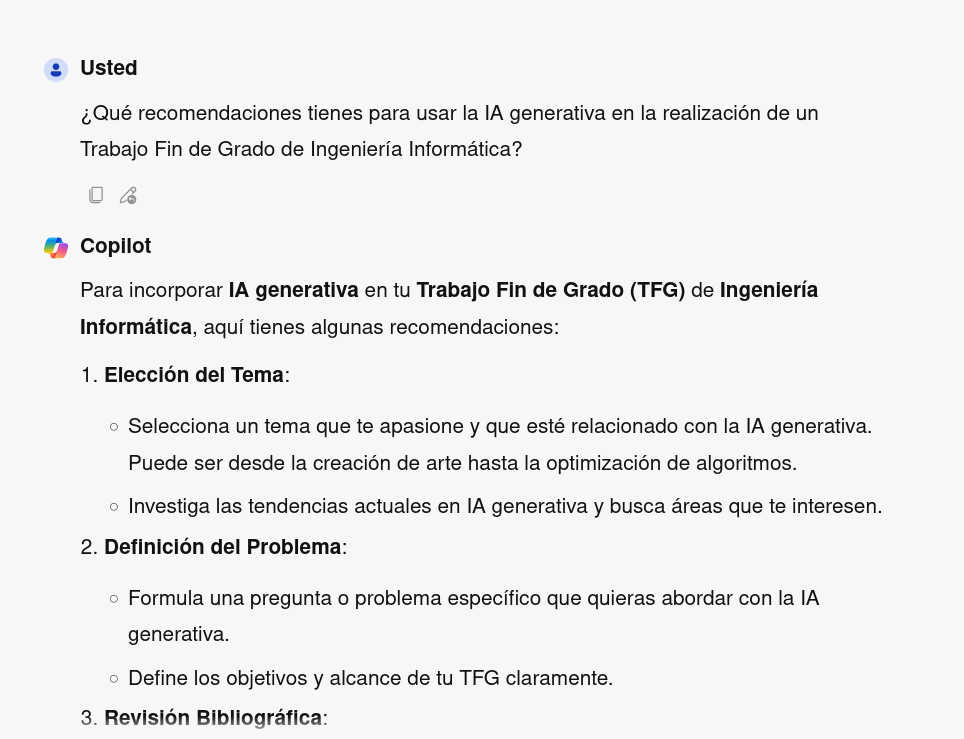
\includegraphics[scale=0.5]{images/Bing.png}
%    \caption{Respuesta (1/3) de Co-pilot de Bing ante la pregunta: ¿Qué recomendaciones tienes para usar la IA generativa en la realización de un Trabajo Fin de Grado de Ingeniería Informática? }
%    \label{fig:Bing}
%\end{figure} 

%\begin{figure}
%    \centering
%    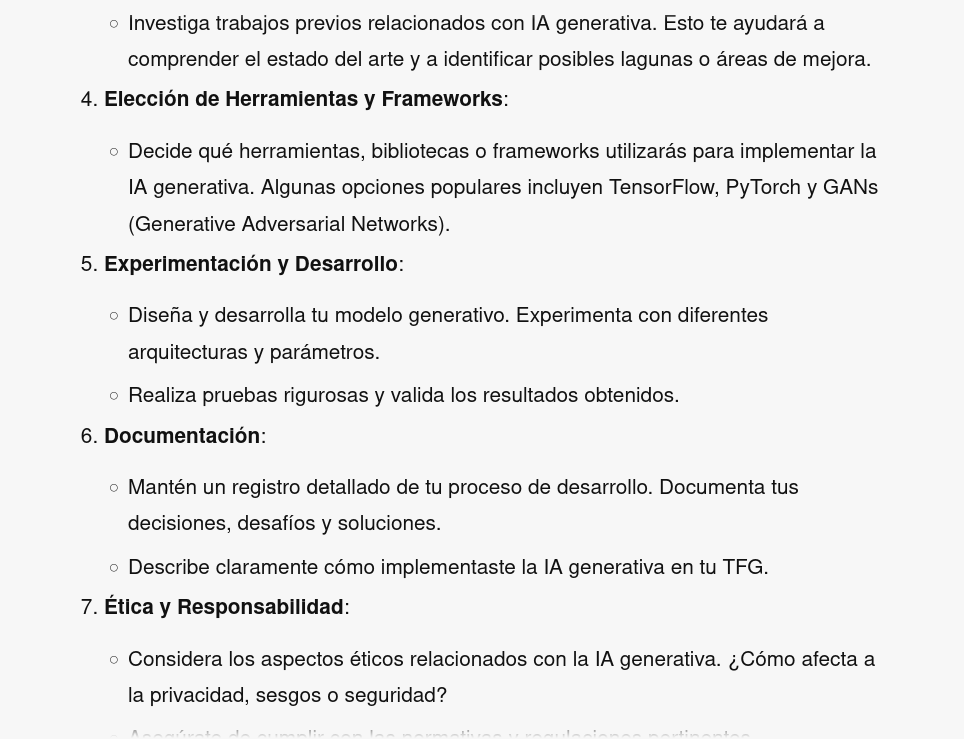
\includegraphics[scale=0.5]{images/Bing2.png}
%    \caption{Respuesta (2/3) de Co-pilot de Bing ante la pregunta: ¿Qué recomendaciones tienes para usar la IA generativa en la realización de un Trabajo Fin de Grado de Ingeniería Informática? }
%    \label{fig:Bing1}
%\end{figure} 

%\begin{figure}
%    \centering
%    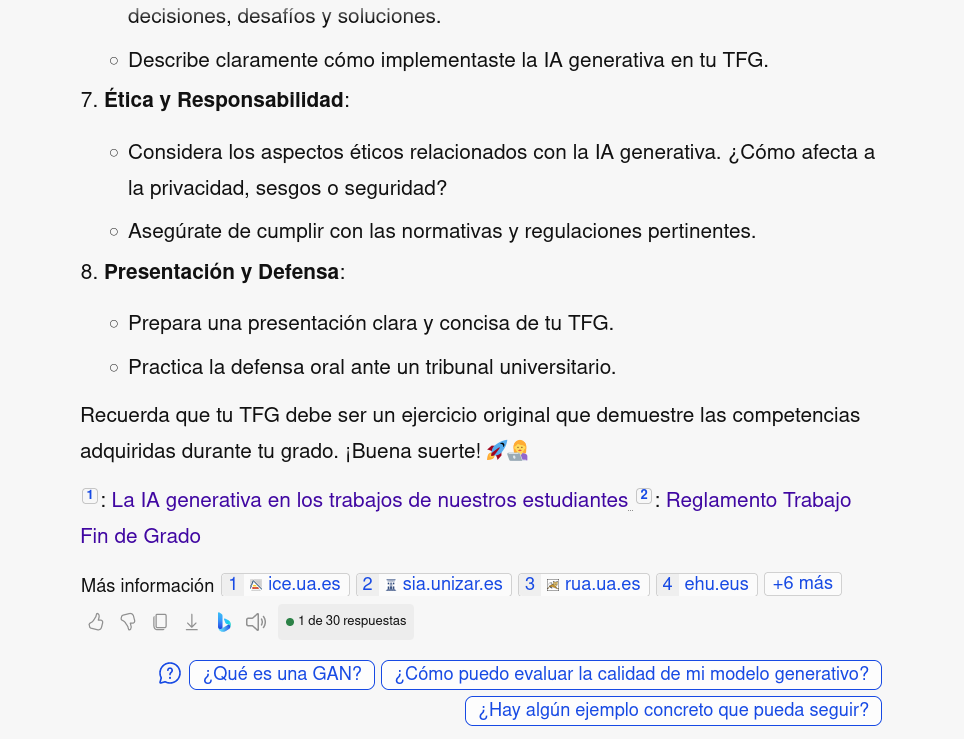
\includegraphics[scale=0.5]{images/Bing3.png}
%    \caption{Respuesta (3/3) de Co-pilot de Bing ante la pregunta: ¿Qué recomendaciones tienes para usar la IA generativa en la realización de un Trabajo Fin de Grado de Ingeniería Informática? }
%    \label{fig:Bing2}
%\end{figure} 

Como última recomendación, pregunta y revisa las directrices que indique tu Universidad, tu centro o tu coordinador del plan de estudios. En el caso de la Universidad de Granada tienes recomendaciones de uso, normativa y herramientas en la web del CEPRUD\footnote{\url{https://ceprud.ugr.es/formacion-tic/inteligencia-artificial}}.

Y recuerda que es tu TFG, apóyate en las IA generativas si lo consideras necesario pero el proyecto es un magnífico ejercicio de aprendizaje y entrenamiento que es bueno que hagas tú en su mayoría.


% Consejos sobre el proceso de desarrollo al estilo de lo que pone María José en sus diapositivas.
% Sobre el código (control de versiones, licencias…) (Aquí puedo ayudar yo (Pablo))
% Sobre cuestiones éticas de código y datos (Alberto).
% Qué cosas hacer y qué no hacer con ejemplos.


%%%%%%%%%%%%%%%%%%%%%%%%%%%%%%%%%%%%%%%%%%%%%%%%%%%%%%%%%%%%%%%%%%%%%%%%%%%%%%
%%%%%%%%%%%%%%%%%%%%%%%%%%%%%%%%%%%%%%%%%%%%%%%%%%%%%%%%%%%%%%%%%%%%%%%%%%%%%%
%Lo consensuado en la reunión del 21/02/24
%%%%%%%%%%%%%%%%%%%%%%%%%%%%%%%%%%%%%%%%%%%%%%%%%%%%%%%%%%%%%%%%%%%%%%%%%%%%%%
%%%%%%%%%%%%%%%%%%%%%%%%%%%%%%%%%%%%%%%%%%%%%%%%%%%%%%%%%%%%%%%%%%%%%%%%%%%%%%

%%%USAR https://docs.google.com/document/d/115O_20YW4Mjx1iJBBxxxDCDWJOBEL_rTzbeHVmI8Cak/edit#heading=h.n5bem9dnws3z


